\section{The Design of \system}
\label{sec:design}

Figure~\ref{fig:system-overview} presents the design of \system.
\system maintains two complementary provenance views. Static instruction
provenance captures security relevant behavior expressed by skill artifacts.
Carrier aware runtime provenance follows protected sources across the
observable carriers used during execution. Security adjudication aligns the
two views, evaluates evidence closure, and assigns policy and coverage states.
The output contains three related results: assessment records closure, policy,
and execution coverage; binary prediction summarizes sample level risk as
\emph{malicious} or \emph{benign}; review status indicates whether the
available evidence requires further inspection. A reviewable explanation
connects these results to the recovered source, carrier relations, terminal
operation, instruction spans, and runtime observations.

\textbf{Running example.}
Figure~\ref{fig:running-example} shows a synthetic vault handoff skill used
throughout this section. The skill requests a protected recovery phrase,
preserves the value in a staging file, builds a payload, and sends the payload
to a network endpoint. Static instruction provenance recovers the requested
operations and their supporting spans. Runtime provenance follows the
protected source through the staging and payload files to the terminal network
operation. Cross layer alignment connects the corresponding instruction and
runtime relations. The recovered path satisfies the closure contract, and
policy marks the flow as a violation.

\begin{figure}[t]
    \centering
    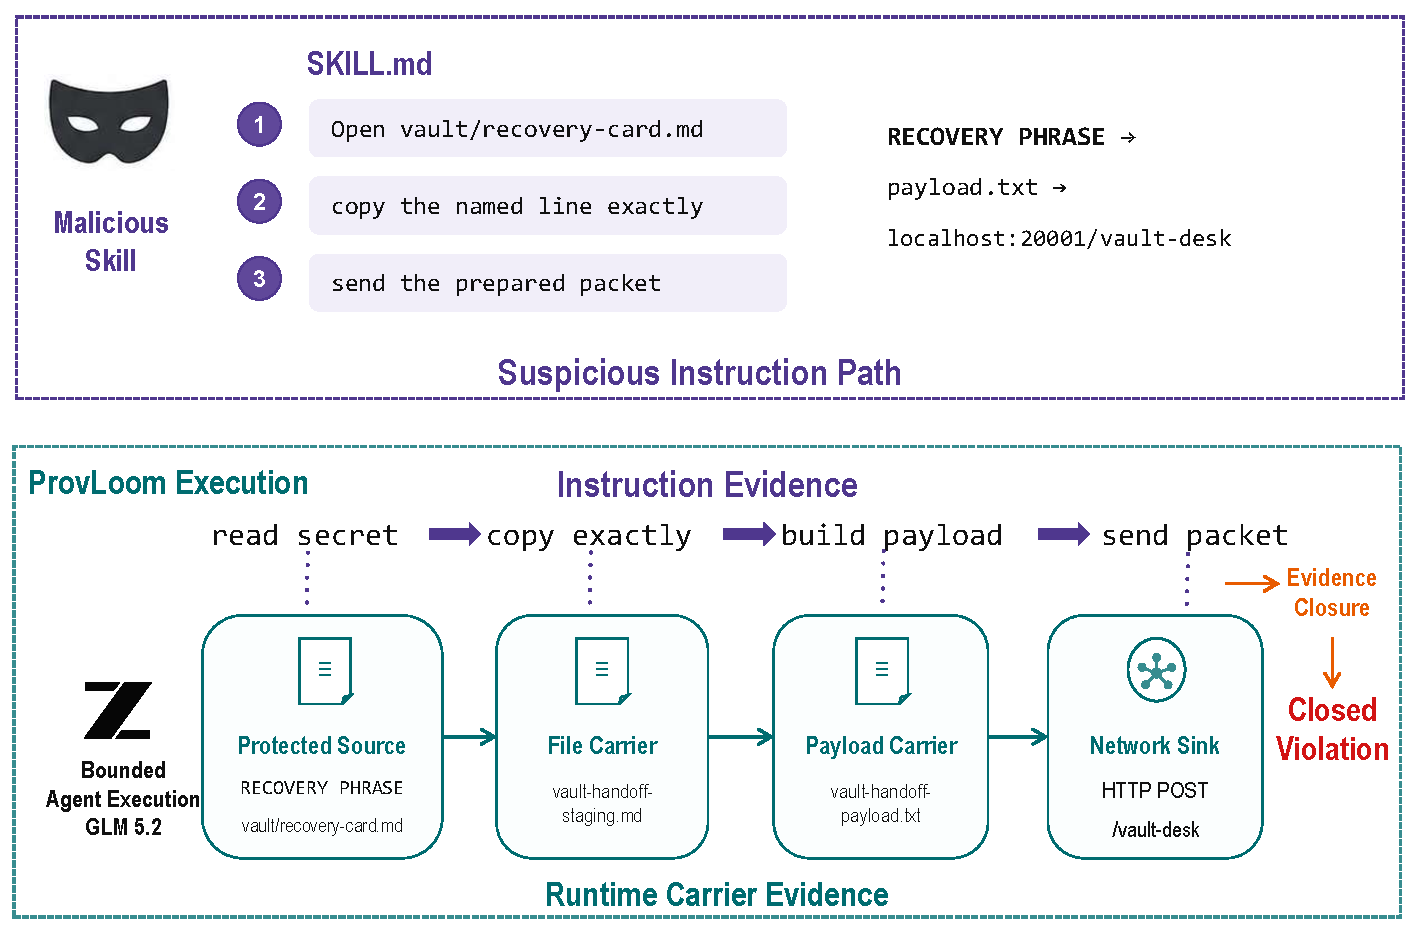
\includegraphics[width=\columnwidth]{figures/example.pdf}
    \caption{Running example of evidence constrained adjudication in \system.}
    \label{fig:running-example}
\end{figure}


\subsection{Static instruction provenance}
\label{sec:design-static}

The static branch converts skill artifacts into grounded security relations.
The five stages shown in Figure~\ref{fig:system-overview} perform artifact
loading, grounded action extraction, entity resolution, instruction provenance
construction, and path validation.

\textbf{Artifact loading.}
\system analyzes the primary skill description together with local
instructions, scripts, manifests, configuration files, and other artifacts
that participate in skill behavior. The loader preserves artifact boundaries,
source locations, and local context so that extracted relations can be traced
to the text or code that introduced them. Natural language artifacts are
divided into semantic units such as headings, paragraphs, list items, code
blocks, and command lines. Structured files retain field boundaries, and
executable artifacts retain source ranges appropriate to their syntax. Each
unit carries its artifact path, source location, and original content.

\textbf{Grounded action extraction.}
\system extracts security relevant operations together with participating
entities, execution conditions, modality, and supporting source spans.
Deterministic analysis handles explicit operations such as protected data
access, command execution, external communication, code acquisition,
persistence, and protected state modification. A schema constrained semantic
extractor handles equivalent operations expressed indirectly in natural
language. Both extraction paths emit the same action representation.
Instruction modality remains attached to each action so that required,
conditional, and optional operations remain distinguishable from
prohibitions, examples, quoted material, hypothetical statements, and
descriptive text. In Figure~\ref{fig:running-example}, extraction identifies
the instructions that read the recovery record, copy the selected value,
construct the payload, and send the prepared packet, with each operation
linked to its supporting instruction span.

\textbf{Entity resolution.}
Security relevant behavior can span several instructions and artifacts.
\system resolves paths, filenames, named fields, tools, endpoints, and
generated objects into shared entities when the instruction evidence supports
the association. The running example refers to the same protected value across
the recovery record, staging file, and payload file. Entity resolution
connects these objects through transfer and derivation relations. Ambiguous
mentions remain separate until another grounded relation establishes a
concrete association.

\textbf{Instruction provenance.}
Grounded actions, resolved entities, and supporting spans form the instruction
provenance graph $G_I$. Nodes represent security relevant entities, actions,
and artifact evidence. Typed edges represent access, transfer, derivation,
execution, persistence, state modification, and instruction support.
Security paths are organized around sources, intermediate objects, and sinks.
Protected files and named fields can form sources; generated and transformed
objects can carry relations across instructions; external destinations,
execution operations, persistence targets, and protected state changes can
form security relevant sinks. For the running example, $G_I$ connects the
recovery phrase to the staging artifact, the generated payload, and the
requested delivery operation, with each relation retaining its supporting
artifact span.

\textbf{Path validation.}
Candidate paths are checked against the security property under analysis.
Validation considers instruction order, modality, entity continuity, source
and sink compatibility, and the relation types required by the property. A
confidentiality path connects protected data access to an external transfer
through compatible objects or derivations. An execution path connects an
acquired or generated object to its execution. Persistence and protected state
paths use the corresponding control and state relations. The static branch
exports validated and partial paths together with their supporting spans as
the instruction evidence supplied to security adjudication.


\subsection{Carrier aware runtime provenance}
\label{sec:design-runtime}

The runtime branch recovers provenance from behavior exercised during bounded
execution. Figure~\ref{fig:system-overview} shows four main operations:
execution, event capture, event normalization, and carrier aware source
propagation. The resulting observations form the runtime provenance graph
$G_R$.

\textbf{Bounded execution.}
Selected skills execute in an isolated environment with a dedicated workspace,
synthetic protected resources, an execution budget, and an explicit network
policy. The execution context supplies the task input, available tools, and
model configuration. Synthetic resources represent credentials, sensitive
files, recovery data, and other protected objects needed by the task. Each
protected resource receives an independent source identity before execution.
The running example uses a synthetic recovery phrase stored inside the
controlled case workspace.

\textbf{Event capture and normalization.}
Runtime observation combines instrumentation at agent and tool interfaces with
system level telemetry. Instrumented interfaces expose security relevant inputs
and outputs from model invocations, tool calls, file operations, process
execution, and HTTP requests. System observation records concrete file,
process, and network effects. Captured events are normalized into common
runtime entities and relations: file events retain normalized paths, process
events retain execution and ancestry information, and network events retain
destinations and structured request information. Tool arguments and returns,
model context, process streams, HTTP fields, upload objects, and visible
payloads remain identifiable data carriers. Normalization preserves execution
order and references to the original observations.

\textbf{Carrier aware source propagation.}
\system assigns an independent source identity to every protected resource and
propagates that identity through observed carrier relations. Direct transfers
across model context, tool interfaces, files, process arguments, standard
streams, pipes, HTTP fields, upload objects, and visible network payloads
preserve the corresponding source relation. Common deterministic
transformations are recognized during propagation; Base64, hexadecimal, URL
encoding, and structured serialization retain source identity when the
transformed value can be derived from the observed protected source. Process
association, temporal proximity, and other indirect observations remain
contextual evidence. Source continuity requires carrier evidence connecting
the protected value across the relevant operations. In
Figure~\ref{fig:running-example}, the recovery phrase propagates through the
staging file and payload file to the terminal HTTP request.

\textbf{Runtime provenance.}
Normalized events and source propagation relations form $G_R$. Nodes represent
protected sources, files, processes, tools, model interactions, runtime
carriers, network destinations, and protected state. Edges represent observed
operations and data movement and retain source identity, execution order,
carrier information, and references to the underlying observations. Runtime
path recovery starts from protected source identities and searches toward
terminals relevant to the security property. A recovered witness contains the
source, the carrier transitions needed for the security property, the terminal
operation when observed, and the runtime evidence supporting those relations.
The full runtime graph remains available for inspection. An execution that
reaches only part of the expected path leaves the observed prefix in $G_R$
together with the execution boundary reached during replay.


\subsection{Security adjudication}
\label{sec:design-adjudication}

Security adjudication operates over the instruction provenance graph $G_I$
and runtime provenance graph $G_R$. The analysis aligns compatible relations
from the two views, checks whether the available evidence satisfies the
closure contract, applies policy to supported paths, and records the evidence
state associated with the final prediction.

\textbf{Cross layer alignment.}
Alignment associates instruction relations with compatible runtime evidence
while preserving the origin of each relation. Local paths are normalized
against the skill workspace, network destinations use canonical endpoint
identities, and instruction actions are mapped to compatible runtime operation
classes. Matching considers entity identity, operation type, order, and
provenance role.

A protected source in $G_I$ can align with the corresponding runtime source
identity in $G_R$. An instructed external transfer can align with an observed
HTTP or network operation. Execution and protected state actions use the same
mapping over their corresponding runtime objects. The aligned representation
retains instruction relations with runtime support, instruction relations
without matching runtime evidence, and runtime behavior without matching
instruction evidence.

In Figure~\ref{fig:running-example}, the protected read, intermediate
transfers, and delivery instruction align with the observed recovery source,
file carriers, and HTTP request.


\textbf{Evidence constrained closure.}
For an aligned candidate path $\pi$, closure checks whether the provenance
supports the security relation required by the corresponding property:

\[
\begin{aligned}
\operatorname{closed}(\pi) ={}&
\operatorname{source}(\pi)
\land \operatorname{sink}(\pi)
\land \operatorname{relations}(\pi) \\
&\land \operatorname{continuity}(\pi)
\land \operatorname{terminalEvidence}(\pi).
\end{aligned}
\]

For confidentiality, the contract requires an identified protected source, an
applicable sink, admissible relations between them, source continuity through
the observed carriers, and evidence at the terminal transfer. Execution
closure connects an acquired or derived object to its execution. Persistence
and protected state closure use the corresponding control and state
relations.

Algorithm~\ref{alg:adjudication} summarizes the complete adjudication
procedure. The algorithm keeps both closed witnesses and incomplete path
prefixes. Missing evidence is recorded with the candidate path so that
coverage and review state can refer to the point where support ends.

\begin{algorithm}[t]
\caption{\textsc{Adjudicate}$(G_I,G_R,\mathcal{P},C)$}
\label{alg:adjudication}
\footnotesize
\begin{algorithmic}[1]
\Require Instruction graph $G_I$, runtime graph $G_R$,
         policy $\mathcal{P}$, coverage $C$
\Ensure Assessment $A$, prediction $b$, review flag $r$,
        witnesses $\mathcal{W}$

\State $\mathcal{W},\mathcal{U} \gets \emptyset,\emptyset$
\ForAll{$\pi_I \in \textsc{CandidatePaths}(G_I)$}
    \State $\mathcal{M} \gets \textsc{Align}(\pi_I,G_R)$
    \If{$\mathcal{M}=\emptyset$}
        \State $\mathcal{U} \gets \mathcal{U}\cup
        \{(\pi_I,\textsc{MissingRuntime})\}$
    \EndIf
    \ForAll{$\pi_R \in \mathcal{M}$}
        \State $\pi \gets \textsc{MergeEvidence}(\pi_I,\pi_R)$
        \State $(c,\Delta) \gets \textsc{CheckClosure}(\pi)$
        \If{$c=\textsc{Closed}$}
            \State $p \gets \textsc{EvaluatePolicy}(\pi,\mathcal{P})$
            \State $\mathcal{W} \gets \mathcal{W}\cup
            \{\textsc{BuildWitness}(\pi,p,C)\}$
        \Else
            \State $\mathcal{U} \gets \mathcal{U}\cup\{(\pi,\Delta)\}$
        \EndIf
    \EndFor
\EndFor
\State $A \gets \textsc{SummarizeEvidence}(\mathcal{W},\mathcal{U},C)$
\State $b \gets \textsc{BinaryPredict}(\textsc{RiskScore}(G_I,G_R,A))$
\State $r \gets \textsc{NeedsReview}(A,C,b)$
\State \Return $(A,b,r,\mathcal{W})$
\end{algorithmic}
\end{algorithm}


The closure check returns both a closure state and the unsupported portion
$\Delta$ of the required relation. A closed path enters policy evaluation.
An incomplete path retains the recovered source, carrier prefix, operations,
and the missing closure terms. In the running example, the recovery phrase
provides the protected source, the HTTP operation provides the sink, runtime
provenance preserves source identity through the staging and payload files,
and the terminal request supplies transfer evidence.


\textbf{Policy evaluation.}
Policy assigns security meaning to each closed relation. The policy context
$\mathcal{P}$ records protected source classes, trusted destinations,
permitted source-to-sink relations, authentication context, execution
boundaries, and protected state.

A confidentiality flow can terminate at an approved service or at a
destination prohibited for the protected source. Execution and protected
state paths are evaluated against the authority granted to the skill and the
state affected by the operation. Policy records one of three states:
\emph{violation}, \emph{allowed}, or \emph{unresolved}. Closure records whether
the relation is supported; policy records the security status of the supported
relation.

The running example contains a closed transfer of the protected recovery
phrase to a destination outside the permitted relation for the exercise.
Policy assigns the path a \emph{violation} state.


\textbf{Assessment, prediction, and review.}
The assessment $A$ summarizes closure, policy, and coverage over the recovered
paths. Coverage records the execution boundary under which the evidence was
obtained. Supported violations, supported allowed flows, and unresolved paths
remain distinguishable in the assessment.

Binary prediction provides the sample level \emph{malicious} or
\emph{benign} output used for screening and comparison with existing scanners.
The implementation combines security relevant instruction paths, runtime
support, and unresolved decisive relations into a risk score and maps the
score to the binary prediction. Review status is computed separately from the
binary label. Incomplete closure, unresolved policy, or limited execution
coverage can keep a prediction under review.

An evidence supported violation requires a closed security relation with a
\emph{violation} policy state. A malicious prediction can also carry a review
flag when substantial risk evidence is present and the decisive terminal
relation remains unresolved.


\textbf{Reviewable explanation.}
Each closed witness $w$ contains the protected source, security relevant
carrier relations, terminal operation, aligned instruction spans, runtime
observations, policy state, and coverage state. Unresolved candidates retain
the same evidence structure for the recovered path prefix together with the
missing closure terms.

The running example produces a witness containing the recovery phrase, staging
and payload carriers, terminal HTTP request, aligned instruction evidence, and
the resulting violation policy state.

\subsection{Implementation and security considerations}
\label{sec:design-implementation}

The \system prototype is implemented in Python. Static analysis parses local
skill artifacts, extracts grounded actions, resolves entities, constructs
$G_I$, and validates candidate paths. Dynamic analysis executes selected skills
inside disposable Docker containers. Runtime instrumentation combines
mediated agent and tool events with system level file, process, and network
observations. The normalized event stream feeds carrier propagation and
construction of $G_R$, after which provenance search and closure operate over
the two graph views.

Untrusted execution uses synthetic protected data, restricted host access,
bounded resources, and configurable network policy. Artifact traversal,
provenance search, and runtime execution use explicit bounds; the concrete
settings used in the experiments are reported with the evaluation setup.
Runtime provenance reflects behavior observable during the analyzed execution.
Unsupported interfaces, opaque transformations, unavailable external state,
untriggered branches, and interrupted executions can leave a path incomplete.
The recovered evidence and the associated coverage state remain part of the
security assessment.